\documentclass[12pt, oneside,titlepage]{article}   	% use "amsart" instead of "article" for AMSLaTeX format

\usepackage{graphicx}
\graphicspath{ {\string} }
\usepackage{subcaption}

%%%%%%%%%%%%%%%%%%%%%%%%%%%%%%%%%%%%%%%%%%%%%%%%%%%%
% set up packages
%%%%%%%%%%%%%%%%%%%%%%%%%%%%%%%%%%%%%%%%%%%%%%%%%%%%
\usepackage{geometry}                
\usepackage{textcomp}                
\usepackage{amsmath}                
\usepackage{graphicx}                
\usepackage{amssymb}                
\usepackage{fancyhdr}                
\usepackage{subcaption}                
\usepackage{bm}                
\usepackage{lineno}

% package for comments
\usepackage{soul}     
\usepackage{setspace}

\usepackage{mathtools}
\usepackage{physics}

%%%%%%%%%%%%%%%%%%%%%%%%%%%%%%%%%%%%%%%%%%%%%%%%%%%%
% call packages
%%%%%%%%%%%%%%%%%%%%%%%%%%%%%%%%%%%%%%%%%%%%%%%%%%%%	
\geometry{letterpaper, marginparwidth=60pt} % sets up geometry              		
\linenumbers % adds line numbers 
\doublespacing % setspace
	
\usepackage[superscript,noadjust]{cite} % puts dash in citations to abbreviate
%\usepackage [autostyle, english = american]{csquotes} % sets US-style quotes
%\MakeOuterQuote{"} % sets quote style

\usepackage{hyperref}
\hypersetup{
    colorlinks=true,
    linkcolor=blue,
    filecolor=magenta,      
    urlcolor=cyan,
}

\usepackage{tabularx}

\usepackage{etoolbox}
\AtBeginEnvironment{quote}{\small}

\usepackage{float,color}
\usepackage{xcolor}
\definecolor{darkspringgreen}{rgb}{0.09, 0.45, 0.27}

\usepackage[section]{placeins}

\usepackage{tikz-qtree}
\usetikzlibrary{trees}

\usepackage{natbib}
%\bibliographystyle{abbrvnat}
\setcitestyle{authoryear}

% Adds parentheses around year
%\setcitestyle{authoryear,open={(},close={)}}


%%%%%%%%%%%%%%%%%%%%%%%%%%%%%%%%%%%%%%%%%%%%%%%%%%%%

%%%%%%%%%%%%%%%%%%%%%%%%%%%%%%%%%%%%%%%%%%%%%%%%%%%%
\pagestyle{plain}                                                      %%
%%%%%%%%%% EXAFT 1in MARGINS %%%%%%%                                   %%
\setlength{\textwidth}{6.5in}     %%                                   %%
\setlength{\oddsidemargin}{0in}   %% (It is recommended that you       %%
\setlength{\evensidemargin}{0in}  %%  not change these parameters,     %%
\setlength{\textheight}{8.5in}    %%  at the risk of having your       %%
\setlength{\topmargin}{0in}       %%  proposal dismissed on the basis  %%
\setlength{\headheight}{0in}      %%  of incorrect formatting!!!)      %%
\setlength{\headsep}{0in}         %%                                   %%
\setlength{\footskip}{.5in}       %%                                   %%
%%%%%%%%%%%%%%%%%%%%%%%%%%%%%%%%%%%%                                   %%		

%%%%%%%%%%%%%
% DEFINE CODE BLOCK
%%%%%%%%%%%%%
\usepackage{listings}

\definecolor{dkgreen}{rgb}{0,0.6,0}
\definecolor{gray}{rgb}{0.5,0.5,0.5}
\definecolor{mauve}{rgb}{0.58,0,0.82}

\lstset{frame=tb,
  language=R,
  aboveskip=3mm,
  belowskip=3mm,
  showstringspaces=false,
  columns=flexible,
  basicstyle={\small\ttfamily},
  numbers=none,
  numberstyle=\tiny\color{gray},
 % keywordstyle=\color{blue},
  commentstyle=\color{dkgreen},
  stringstyle=\color{mauve},
  breaklines=true,
  breakatwhitespace=true,
  tabsize=3,
  otherkeywords={0,1,2,3,4,5,6,7,8,9},
  deletekeywords={data,frame,length,as,character,dunif,ps},
}

%%%%%%%%%%%%%%%%%%%%%%%%%%%%%%%%%%%%%%%%%%%%%%%%%%%%
\usepackage{tikz}
\usetikzlibrary{arrows,automata}
\usetikzlibrary{positioning}

\usepackage{pgfplots}
\usepgfplotslibrary{groupplots,fillbetween}
\usepackage{animate}

%%%%%%%%%%%%%%%%%%%%%%%%%%%%%%%%%%%%%%%%%%%%%%%%%%%%

%\usepackage{todonotes}

\begin{document} 

%%%%%%%%%%%%%%%%%%%%%%%%%%%%%%%%%%%%
% TITLE PAGE
%%%%%%%%%%%%%%%%%%%%%%%%%%%%%%%%%%%%
\begin{titlepage}
   \begin{center}
       \vspace*{1cm}
 
       \textbf{Resources and development jointly shape life history evolution in plants}
 
       \vspace{1.5cm}
 
       Gregor-Fausto Siegmund, Stephen Ellner, Monica Geber
 
   	Last updated: \today
 
   \end{center}
\end{titlepage}


%%%%%%%%%%%%%%%%%%%%%%%%%%%%%%%%%%%%
% INTRODUCTION
%%%%%%%%%%%%%%%%%%%%%%%%%%%%%%%%%%%%
\section{Introduction}

\singlespace
\begin{itemize}

\item The interplay between development and ecology is the basis for evolutionary change [evolution is the control of development by ecology (van Valen)]

\begin{itemize}
\item A central tenet of life history theory is that selection maximizes fitness by favoring trait combinations that optimally balance different parts of the life cycle (\cite{cole1954,lande1983}). 
\item Theoretical and empirical studies typically assume that organisms must allocate a limited pool of resources to competing functions such as growth versus survival. \cite{fox1990} states this assumption is shared by approaches of reproductive effort, dynamic optimization, and evolutionary demography. Quantitative genetics assumes that there are correlations among components of life history but focuses on genetic and phenotypic correlations.
\item From early papers that used optimal control theory to study life history evolution, authors have suggested incorporating development into the models (\cite{cohen1971,schaffer1982,fox1992a}). However, no such models have yet been developed. 
\end{itemize}

\item Multiple lines of evidence support the association between life history and architecture

\begin{itemize}
\item Adaptive radiations on oceanic and sky islands demonstrate association between life history and morphology in shift from annual/herbaceous to perennial/secondary woodiness \cite{nurk2019}
\item Developmental biology: studies demonstrate how maintenance of active apical or axillary meristems changes architecture and life history. Includes comparisons such as mutant lines of model plants, comparisons of genes between annual/perennial relatives (\cite{remington2015,ponraj2020})
\item Evolutionary ecology studies in the field demonstrate the role of branching in life history as well; examples include ecotypes of Mimulus guttatus (\cite{baker2011,baker2014,friedman2015a}), Erysimum populations across an elevation gradient (\cite{kim2011})
\item \hl{Identify studies that demonstrate the presence of heritable genetic variation in bud differentiation/organ identity}. For example, potentially could include \cite{bonser1996,bonser2003,doust2006,baker2012,huang2013,baker2014,rubin2018}. Could also cite crop studies (e.g. \cite{hardy1998})
\end{itemize}

\item Various lines of evidence exist that point to constraints of development on life history evolution that should inform optimization studies 

\begin{itemize}
\item Experiments that show genetic covariance/correlation of flowering time and meristem number/tiller number. We have data from plants from different habitats (e.g. \cite{geber1990a,schmitt1993}), from RILs (e.g. \cite{haselhorst2011}), from the result of selection experiments (e.g. Mitchell-Olds 199x?). Also \cite{watson1984a,vantienderen1996,duffy1999,kudoh2002,friedman2015a} Diggle 1993, Gardner and Latta 2008, Latta and Gardner 2009, Austen et al.  2014, Rubin et al. 2018
\item Studies of development with mutants/knock-outs in Arabidopsis that show that modifying flowering time genes (e.g. tfl) has an effect on the number of meristems, establishing that there is pleiotropy (\cite{bradley1997,karami2020}, Melzer et al. 2008, Baumann et al. 2015)
\item We have studies focusing on developmental stages (e.g. \cite{baker2011}). 
\item \cite{parker1990} describe how comparative studies and quantitative genetics can be used in conjunction with optimization to understand phenotypes. Specifically, they suggest that quantitative genetics can be used to identify constraints that are relevant for optimization models. Comparative methods can then  be used to test the predictions of those models. Here's a quote: "discovery of a genetic covariance can indicate presence of a developmental constraint that must be taken into account when formulating an optimization model". Experiments and interspecies comparisons can also help discover these constraints. 
\end{itemize}  

\item Plant growth and development

\begin{itemize}
\item Plants grow and reproduce via meristems, tissues that are made up of undifferentiated cells and are analogous to stem cells in animals (reviewed in \cite{mcsteen2005,wang2018}).
\item Individual meristems can grow vegetatively, become an inflorescence meristem, or remain undifferentiated. Each vegetative meristem may generate additional meristems with the potential to differentiate into one of these three types. A meristem that differentiates into an inflorescence can no longer grow vegetatively. The onset of flowering thus prevents future vegetative growth at the level of individual meristems.
\item Limiting the number of meristems available for differentiation and reproduction can thus produce tradeoffs: a plant with that allocates most of its meristems to reproduction now will not be able to allocate those meristems to reproduction later (\cite{watson1984a,geber1990a,schmitt1993}).
\end{itemize}

\item Theory and models identify consequences of variation in season length on resource allocation decisions

\begin{itemize}
\item For a fixed season length (no variability), a bang-bang control maximizes arithmetic mean fitness (\cite{cohen1971})
\item For a uniform distribution of season length (highly variable), the optimization problem becomes one of maximizing geometric mean fitness. In this case, simultaneous allocation to vegetative and reproductive growth can be part of optimal strategy (\cite{king1982a}). 
\item Using an evolutionary algorithm and examining intermediate variability in season length (between fixed and uniform distribution), the authors find that steepness of gradient relates to the amount of variability in the environment (\cite{wong2005}). 
\item A study that examines the production of workers versus sexual individuals in annual eusocial insects suggests that high levels of environmental variability are required to promote a graded control; they propose that realistic levels of environmental variability in season length are unlikely to be sufficient to do so; complements study above (\cite{mitesser2007}).
\item Variations on the basic form of the model explore the effect of mortality (\cite{cohen1976}), nonlinear (\cite{vincent1980}) or seasonal production functions (\cite{schaffer1982,fox1992}), tissue loss (\cite{king1982}), storage (\cite{chiariello1984}), or constrained growth (\hl{citation needed}).
\item More thoughts? Overview of model types that address connection of life history and timing or reproduction. Specific benefits of optimal control. Original models have been extended and enriched. I think this should be reduced to 1-2 concise paragraphs that also address other modeling approaches that have been used to study this kind of problem (evolutionary algorithms; \cite{wong2005}) and why we chose to use optimal control theory.
\end{itemize}

\item Branching modifies plant architecture and contributes to temporal patterns of resource allocation and reproduction

\begin{itemize}
\item A model of development demonstrates that season length and variability determine the optimal morphology of an inflorescence. (\cite{prusinkiewicz2007}). Ideas presented in this confirmed in tomato by a study demonstrating that inflorescence architecture is determined by rate of meristem maturation (\cite{park2012}).
\item Variety of evidence associating variation in branching with environment: branching and altitude (\cite{milla2008}), bud banks increase with productivity in perennials (\cite{dalgleish2005})
\item Developmental programs differ among plants in terms indeterminate versus determinate flowering, and how is that related to resource allocation patterns
\item Developmental genetics identifies independent/related basis for flowering time, leaf production, and growth rate. Review to determine what these studies state about the relationship among these variables (e.g. \cite{rao2008,melzer2009,mendez-vigo2010,remington2013,serrano-mislata2016,moraes2019,taylor2019,karami2020})
\item Inflorescence unit number and size; increasing total flower number impacts RS through both genders;  \cite{fishbein1996}
\end{itemize}

\item Past examination of branching and allocation/bet hedging

\begin{itemize}
\item \cite{pyke1989,kudoh2002,suzuki2006,hughes2014a}
\end{itemize}



\end{itemize}
\doublespace


Life history theory is a framework for understanding how evolution generates and responds to tradeoffs among growth, survival, and reproduction over the course of an organisms' life cycle. A central tenet of life history theory is that selection maximizes fitness by favoring trait combinations that optimally balance different parts of the life cycle (\cite{cole1954,lande1983}). Theoretical and empirical studies typically assume that organisms must allocate a limited pool of resources to competing functions such as growth versus survival. While this may be an appropriate assumption for animals, plants are modular organisms.

Plants grow and reproduce via meristems, tissues that are made up of undifferentiated cells and are analogous to stem cells in animals (reviewed in \cite{mcsteen2005,wang2018}). Individual meristems can grow vegetatively, become an inflorescence meristem, or remain undifferentiated. Each vegetative meristem may generate additional meristems with the potential to differentiate into one of these three types. A meristem that differentiates into an inflorescence can no longer grow vegetatively. The onset of flowering thus prevents future vegetative growth at the level of individual meristems. Limiting the number of meristems available for differentiation and reproduction can thus produce tradeoffs: a plant with that allocates most of its meristems to reproduction now will not be able to allocate those meristems to reproduction later (\cite{watson1984a,geber1990a}).

In plants where reproduction is fatal (monocarpic plants), plants must balance their investment in and the timing of growth and reproduction because both processes draw on a shared set of resources. Theoretical models of life history evolution typically represent this as a trade-off in energetic investment. However, plant development is modular and can constrain future energetic allocation to growth or reproduction.

\hl{The hypotheses I've written turn explicitly to developmental patterns. I think that the question has become more about the relationship between development and the environment than it was when I originally wrote this introduction. It would be helpful to have theory about the relationship of development, evolution, and ecology (e.g. Dahlem Konferenz 1981) and empirical examples from other systems/organs (Sultan? toads?)}

\cite{fox1990} discusses experiments with Eriogonum demonstrating that patterns of reproduction are the product of growth and development. 

%%%%%%%%%%%%%%%%%%%%%%%%%%%%%%%%%%%%
% QUESTIONS
%%%%%%%%%%%%%%%%%%%%%%%%%%%%%%%%%%%%
\subsection{Questions}

\singlespace
\begin{itemize}

\item Questions for an unbranched plant with a determinate inflorescence (1-dimensional model with a switch time only)
\begin{itemize}
\item ...
\end{itemize}

\item Questions for a branched plant with a determinate inflorescence
\begin{itemize}
\item Are plant life histories more sensitive to meristem or resource constraints in face of variability in season length? When season length is variable, branching creates variation in meristem number that in turn supports simultaneous growth and reproduction, and may be a a strategy that reduces variability in fitness. 
\item How do meristem and resource constraints shape life history? Meristem and resource constraints will both influence fitness; the optimal strategy will be determined by the relative magnitude of the rate of meristem divisions and resource use efficiency.
\end{itemize}

\item Questions about optimal control
\begin{itemize}
\item I will use the models to determine whether including differentiation and growth of meristems reduces the likelihood of obtaining a strategy with an instantaneous switch (\cite{cohen1971}). Put another way, are graded allocation strategies optimal when vegetative and reproductive growth are coupled \cite{fox1992a}? 
\item I will look at the control strategies of decisions (e.g. meristem division) and the cumulative impact on control of resource budget. Do the control strategies of meristem decisions (e.g. bang-bang) translate to resource budgets (also being bang-bang?) (\cite{fox1992a})? 
\item I will ask when plants are more likely to be resource versus meristem limited. Specifically, I will focus on how the optimal strategy changes with increasing levels of environmental variation; are plants likely to be meristem limited in scenarios with high levels of uncertainty about season length in order to maintain the ability to capitalize on those longer seasons? (\cite{wyatt1982,schemske1980,stebbins1974,salomonson1994})
\end{itemize}

\item Questions about the optimal strategies under different allocation rules
\begin{itemize}
\item What is the best strategy when there are no meristems? 
\item What is the best strategy when the rates are the same but there are meristems? 
\item A model of resource allocation decisions will inevitably produce trade-offs that are the result of resource limitation. Will a model of meristem allocation decisions inevitably produce trade-offs that are the result of meristem limitation? 
\end{itemize}

\item Distinguish meristem versus resource allocation as the trade-off shaping life history evolution.
\begin{itemize}
\item Geber, Fox, Lehtila and Larsson
\item Define conditions for meristem vs. resource limitation.
\item Set up boundary conditions or test cases that demonstrate meristem vs. resource limitation.
\end{itemize}

\item Does including development lead to bang-bang control or graded allocation, and how does this depend on development mode?
\begin{itemize}
\item Hypotheses: Cohen, King and Roughgarden, Fox, Iwasa 
\item Recover optimal controls.
\item Compare results to the strategies from the Cohen or King and Roughgarden models. 
\end{itemize}

\item Explore the effect of environmental variation on flowering time via development.
\begin{itemize}
\item Hypotheses: \cite{wyatt1982,stebbins1974,prusinkiewicz2007}
\end{itemize}

\item Predictions about season length and variability in season length
\begin{itemize}
\item I expect that longer seasons favor branching (\cite{geber1990a}). 
\item As the end of the season becomes more unpredictable, it might become advantageous to have multiple branches, some of which can produce flowers and others which might still be producing leaves (\cite{geber1990a}). 
\item  I also expect this effect to be less pronounced for plants which produce inflorescences than single flowers (\cite{bonser2006}), as inflorescences should provide additional flexibility in how many flowers to produce per reproductive meristem (\cite{bonser2006,salomonson1994}).
\item "a particular plant morphology is the product of developmental decisions about the number and types of metamers, and thus branches produced. Is carbon availability critical to such decisions, and if so, at what level of morphological organization is its availability assessed?" 
\item Developmental decisions are made so as to maintain a positive carbon balance within a physiological  unit (\cite{watson1984}). When reproductive and vegetative branch formation compete for the same meristems, the development of reproductive branches will reduce the number of vegetative branches that can form (\cite{watson1984a}). Even if reproductive branches may be able to support themselves, forming them may reduce ultimate carbon balance because they are unlikely to contribute excess assimilate. Life history theory for animals does not apply to plants - the assumptions are not valid for plants where elaborating the aboveground structure can pay for its own cost. "predictions about a plant's behavior in different environments will vary according to the time period in which carbon availability acts as a developmental constraint, the degree to which translocation of assimilate is architecturally constrained, and the extent to which structures differ in their capacity to be carbon-autonomous." (\cite{watson1984}).
\item Flowering in plants is correlated with rosette size - does this reflect the availability of stored assimilate to support maturation of the inflorescence OR does it reflect the development of sufficient leaves to support the inflorescence with current assimilate?
\end{itemize}

\item Predictions in terms of model parameters

\begin{itemize}

\item When does flowering start? This asks when plants start allocating meristems to reproduction, or when plants start producing inflorescence meristems. In the model for determinate inflorescences, this would be when $ p(t) < 1 $. In the model for indeterminate inflorescences, this would be when $ p(t) - q(t) < 1 $ or $ q(t) > 0$.

\item How quickly do plants commit resources to flowering? This asks whether there is an instantaneous or graded allocation to reproduction.

\item How do allocation strategies respond to different levels of interannual variation? How does the optimal control shift with increasing variance in season length? % has the flavor of comparing bifurcation diagrams - at what points do you get changes in qualitative behavior - not testing any particular number or trajectory but the qualitative changes tha occur as you tune parameters - when you shift from one type of behavior to another is a good way of comparing models

% \item also think about when the constraints become active - what does it take to get yourself in a situation where those constraints are active - should they be doing that all the time vs. not

% \item could compare constraint on rates vs. constraint on allocation (should be always active) vs. states

\item  How do optimal strategies respond to different rates of division in primary and inflorescence meristems, $\beta_1$ and $\beta_2$? For example, what is the optimal control for different levels $\beta_1<\beta_2$ (primary meristems divide more slowly than inflorescence meristems), $\beta_1=\beta_2$ (primary and inflorescence meristems divide at equal rates), or $\beta_1>\beta_2$ (primary meristems divide more quickly than inflorescence meristems)?

\item What is resource limitation in these models? What is meristem limitation in these models? 

\item Which developmental mode favors meristem limitation? MAG suggest that determinate development should favor meristem limitation because the meristem can be consumed by a floral meristem while indeterminate development can always keep growing.

\item When are resource allocation models appropriate for understanding the developmental decisions that plants make? When are resource allocation models insufficient for understanding the developmental decisions that plants make?

% \item Hypothesis: species with indeterminate flowering may have stronger apical dominance when undamaged than species with determinate flowering when undamaged. Indeterminate flowering species may thus show stronger compensatory responses than determinate flowering species. (Adhikari Russell 2014). This could be tested by selecting for an optimal strategy under no herbivory for undamaged vs. damaged species, and then tracking how the strategy responds to imposing herbivory. This might work if the probability of meristem division is lower (stronger apical dominance) in indeterminate flowering species and the probability of meristem division is higher (weaker apical dominance) in determinate flowering species. 

% \item  Weak apical dominance = higher probability of meristem division. Increase in resources would break dominance and activate axillary meristems. (Wise Abrahamson)

% \item Indeterminate flowering: flexibility in number of flowers in the apical inflorescence up to amount enabled by increase in resources. (Wise Abrahmson)

\end{itemize}

\item More predictions about flowering time and meristems
\begin{itemize}
\item Early flowering reduces meristem number and late flowering increases meristem number. 
\item Environmental risk (e.g. dry habitats) promote the evolution of annuals and early flowering. This could be an interspecific comparison (within genera) or intraspecific (populations in riskier habitats flower earlier). 
\item Annuals derive from perennial ancestors (phylogenetic).
\end{itemize}

\end{itemize}
\doublespace







\subsection{Overview of dynamic optimization (assumptions, predictions, goals)}

Life history theory typically assumes that trajectories of growth and reproduction are shaped by resource allocation decisions. Descriptions of development (Figure \ref{fig:transitions-determinate} and \ref{fig:transitions-indeterminate}) highlight how growth and fecundity depend on meristem production. Models that do not explicitly represent resource and development can not distinguish between the origin of tradeoffs. See \cite{white2016} for a complementary perspective on sources and sinks in plant growth and \cite{korner2015} for a review on how sinks might often limit plant growth. \cite{fox1992a} suggests allometric models are not sufficient and models that incorporate development will be necessary.

A key assumption of the classic models is that plants are making allocation decisions about carbon, which is assumed to be the limiting resource. Although this assumption has been extended to include other nutrients, plant development complicates the picture. Because plants have modular structures, vegetative and reproductive growth are coupled insofar as plant architecture limits the total potential number of flowers or inflorescences. More generally, whether a plant is in a vegetative or reproductive phase is the product of decisions about the fate of primary or axillary meristems. This perspective aligns with a source-sink perspective on plant growth that suggests potential photosynthesis is not the sole determinant of plant growth but that plant growth is instead a balance of source (photosynthate) and sinks (maintenance, organ production, etc.) \cite{korner2015,white2016}.

A shared assumption of reproductive allocation models, dynamic optimization models, and evolutionary demographic theory is that demographic parameters are themselves parts of organisms (\cite{fox1990}, p 1420). However, the representation of organisms in these models is nonetheless an abstraction. In particular, they treat growth and reproduction as independent components of an organism's life history to which some fraction of a limiting resource can be allocated. (\cite{fox1990}, p 1407) outlines three key points to why its important that development couples reproduction and growth for understanding how plants respond to drought. First, the models above assume that the reproduction and growth are independent. Second, developmental coupling is invariant among populations suggesting similar responses to the environment. 

Modifications to original models include varying functions for productivity and reproduction (e.g. seasonal pattern, overlap or not), tissue loss and maintenance costs, multiple organs, allocation to storage, different types of survivorship curves, allometric relationships of reproductive to vegetative mass, and environmental stochasticity. The value in these models comes from an ability to explore how allocation decisions respond to different assumptions about variables such as resource use or variability in season length. 

\singlespace
\begin{itemize}

\item Cohen 1971: derives bang-bang control; maximizes arithmetic mean yield; does not derive analytical solution for maximizing geometric mean
\item Cohen 1976: constant environment, maximize arithmetic mean, ... [what are key conclusions here?]; also considers describing survival by a decreasing function and finds bang-bang
\item Vincent and Pulliam 1980: analyzes Cohen 1971, generalizes the model; considers 2 photosynthate production functions (linear + nonlinear, saturating), both predict bang-bang; also analyzes optimal leaf toxin allocation
\item Schaffer, Inouye, Whittam 1982: seasonal variation in photosynthesis/storage
\item King and Roughgarden 1982: introduces random variation in season length; maximizes geometric mean fitness; builds on C71; obtains graded control, basis for Fox 92, Lindh 16
\item King and Roughgarden 1982: includes tissue loss (herbivory); Rathcke and Lacey (84) claim as accurate
\item Chiariello and Roughgarden 1982: includes tissue loss (herbivory), seasonal variation in assimilation/storage
\item Fox 1992: modifies photosynthate production function to be time-varying (with a peak) and looks at different survivorship curves
\item Fox 1992: reviews assumptions of resource allocation models; develops allometric model (cf Lindh 2016); suggests development needs to be incorporated
\item Shitaka and Hirose 1993:
\item Johansson et al. 2013: "the seasonal distribution of productivity (e.g. temperature and precipitation) can affect the size and even the direction of the optimal response of the flowering time to certain types of environmental change, such as increased productivity or increased season length" (Lindh et al. 2016), "assumed that plant growth rate is proportional to the vegetative mass during the growth season" (Lindh et al. 2016)
\item Lindh et al. 2016: modifies KR82 by making growth exponential, logistic, or WBE (general constrained or allometric); also in appendix shows bang-bang control with exponentially decreasing survival corresponding to constant mortality

\end{itemize}
\doublespace

\section{General approach}

\singlespace
\begin{itemize}
\item Describing plant development and branching using differential equations

\begin{itemize}
\item Various authors have proposed considering plants as a population of subunits (e.g. \cite{white1979}).
\item Plant architecture can be described using L-systems (\cite{prusinkiewicz2007}) but here we do not explicitly represent branching but rather the population of plant parts that result from branching. This is analogous to an approach modeling cell divisions using differential equations (\cite{itzkovitz2012}).
\end{itemize}

\item We developed differential equations that capture the basic processes of plant development 

\begin{itemize}
\item Assumed key step limiting steps were \hl{review} (\cite{fox1992})
\item Followed dichotomous characterization of inflorescence development (\cite{kellogg2000}
\item Key transition was from producing vegetative to inflorescence meristems, as suggested by developmental studies (e.g. \cite{bradley1997}).
\item Interpretation of conversion efficiency is based on physiological interpretation (\cite{ackerly1999})
\item Interpretation of per-capita rate of meristem division is based on plastochron index
\end{itemize}

\end{itemize}
\doublespace

We took the following approach to solving the problem outlined above. First, we sought to develop differential equations that capture the basic processes of plant development that are relevant to our questions. To accomplish this goal, we reviewed existing literature on plant development, models of plant development. Second, we specified the optimal control problem and goals. This step included defining Hamiltonian for cases with and without state variable constraints. Third, we solved the optimal control for the case without state variable constraints. We took this step in order to develop intuition about the system and to determine initial conditions for the numerical solution. Finally, we implemented a numerical algorithm to obtain solutions to the optimal control problem. 

Here, we apply these ideas to develop a system of ordinary differential equations that describes the dynamics of plant development and constrains growth by the availability of photosynthate. This approach places the allocation decisions at the level of meristems (decisions about meristem fate) and leaves flexibility about much these decisions are limited by photosynthate. In classic models, any quantity of vegetative biomass can support unlimited primary meristem divisions which can in turn  contribute to unlimited number of floral meristems.

Resource limitation generates negative correlations between growth and fecundity within a life stage because both compete for resources. In a situation where resources are limited, we might expect to see trade-offs that are the result of resource allocation decisions (we wouldn't see these decisions when resources are not limited).

Meristem limitation generates positive correlations between growth and fecundity within a life stage because both depend on meristem production. In a situation where meristems are limited, we might expect to see trade-offs that are the result of meristem allocation decisions (we wouldn't see these decisions when meristems are not limited). 

Goals: connect vegetative branching, inflorescence development, trade-offs, and flowering time. Distinguish meristem versus resource limitation as the trade-off shaping life history evolution. Explore the effect of environmental variation on flowering time via development. Does including development lead to bang-bang control or graded allocation, and how does this depend on development mode.

\section{Models of plant development}

\hl{ The description of plant development that I give here should be directly connected to a figure demonstrating the different types of divisions that I base the model on. The file basic-inflorescence in the notes folder should be helpful for this. I think I need to make the case that the interplay between meristem and resource allocation are well-represented by two basic developmental decisions: whether or not the plant branches, and whether the inflorescence is determinate or indeterminate. I will try to marshal: (1) a brief overview of research on genetics of development, (2) role of these processes in shaping plant morphology, (3) life history arguments. }

Development in flowering plants can be characterized as a series of decisions at the meristems \cite{kellogg2000}. The primary shoot divides at the shoot apical meristem (SAM) and produces additional primary shoot meristems (main branch) and axillary meristems (AM), each of which is subtended by a leaf. The axillary meristems can develop into an axillary branch or remain quiescent. Each axillary branch has similar dynamics as the primary shoot meristem (though potentially at different rates). The shoot apical meristem is converted to an inflorescence meristem (IM) through internal or external signals. In turn, inflorescence meristems give rise to floral meristems (FM). 

In plants with determinate inflorescences, the inflorescence meristem is eventually converted to a terminal flower, which consumes the meristem. Tomato is an example of a plant with a determinate inflorescence and sympodial growth \cite{park2012}. In plants with indeterminate inflorescences, the inflorescence meristem only produces flowers at axillary positions. \textit{Arabidopsis} is an example of a plant with an indeterminate inflorescence and monopodial growth \cite{bradley1997}. 

The `rules' characterizing plant development have been used to model the evolution of inflorescence architecture \cite{prusinkiewicz2007}. The meristem dynamics that underly inflorescence architecture are also likely involved in organizing branching architecture \cite{park2012}. Lindenmayer systems (L-systems) are a grammar that is capable of reconstructing the branching architecture of various organisms (e.g. algae, bacteria, plants). L-system statements highlight the overlap in decision rules that determine branching in vegetative and reproductive growth. 

\cite{cohen1971} identified development as a factor that could help explain why an instant switch in allocation from vegetative to reproductive growth is rarely observed. Development connects growth and reproduction, and constrains how plants can shift allocation to reproduction \cite{fox1992a}. Life history models for plants have not included developmental processes, which may limit their applicability and interpretation \cite{fox1992a}. For example, it may be easier to test the predictions from models that separate meristems and biomass. Also, models that do not represent development can not determine whether allocation patterns are the result of selection on developmental decisions or resource allocation directly. The broader issue here is whether resource-based models can adequately represent plant life histories, or whether it is necessary to include development to describe the biological processes underlying life histories \cite{fox1992a}. \hl{need to work on this paragraph}

I first describe resource allocation models \cite{cohen1971,king1982a}. I then describe how I represent meristem and resource allocation in models for plant life histories. These models are developed from ideas in \cite{fox1992a,kellogg2000,prusinkiewicz2007,itzkovitz2012}. First, I write models for plants with determinate inflorescences. Next, I write models for plants with indeterminate inflorescences. 

%The main branching systems that are present in nature are monopodial and sympodial. In monopodial systems, the apex remains active. In sympodial systems, the apex terminates at some point. 

\section{Determinate inflorescences}

In plants with determinate inflorescences, the shoot apical meristem forms a terminal flower and an axillary bud \cite{bartlett2014}. In tomato, the primary shoot meristem converts to a floral meristem and a sympodial inflorescence meristem; this pattern is iterated to form the inflorescence \cite{park2012}. 

I describe the developmental decisions in a plant with determinate inflorescences using three types of divisions (Figure \ref{fig:transitions-determinate}) \cite{itzkovitz2012}. First, a primary meristem can divide at the shoot apical meristem to give rise to two primary meristems: the main branch and an axillary bud. These divisions generate a vegetative, branching architecture. Second, a primary meristem can divide at the shoot apical meristem to give rise to an inflorescence meristem and a floral meristem. These divisions end vegetative growth and mark the transition from vegetative to reproductive growth along an axis. Third, an inflorescence meristem can divide into an inflorescence meristem and a floral meristem. These divisions are the only possible fate for inflorescence meristems. Using these categories assumes that there is no terminal division into two floral meristems. The end of season terminates flowering. This assumption is somewhat unrealistic because some plants do stop flowering. 


\begin{figure}[hbt!]
  \begin{subfigure}{.25\textwidth}
  \centering
    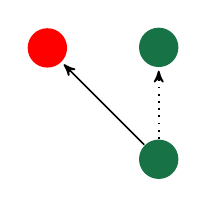
\begin{tikzpicture}[->,>=stealth',shorten >=1pt,auto,node distance=2cm,
                    semithick]
  \tikzstyle{every state}=[draw=none]

  \node[state, fill=darkspringgreen,minimum size=.5cm] 	     (A)                    {};
  \node[state, fill=red,minimum size=.5cm]         (B) [above left of=A] {};
  \node[state, fill=darkspringgreen,minimum size=.5cm] 	     (D) [above = .9cm of A]                   {};

  \path[dotted] (A) edge              (D);
  \path[->] (A) edge (B);

      \end{tikzpicture}
          \caption{Primary meristem transitioning to one vegetative meristem and generating two primary meristems.} 
  \end{subfigure}
              \hspace{\fill}
             \begin{subfigure}{.25\textwidth}
    \centering
    \centering

      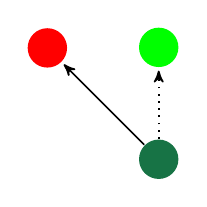
\begin{tikzpicture}[->,>=stealth',shorten >=1pt,auto,node distance=2cm,
                    semithick]
  %\tikzstyle{every state}=[fill=red,draw=none,text=white]

  \node[state, fill = darkspringgreen, draw = none,minimum size=.5cm] (A)                    {};
  \node[state, fill = red, draw = none,minimum size=.5cm]         (B) [above left of=A] {};
  \node[state, fill=green, draw = none,minimum size=.5cm] 	     (D) [above =.9cm of A]                   {};

  \path[dotted] (A) edge              (D);
  \path[->] (A) edge (B);

      \end{tikzpicture}
    \caption{Primary meristem transitioning to one vegetative meristem, and generating inflorescence and floral meristems.}
      \end{subfigure}
          \hspace{\fill}
      \begin{subfigure}{.25\textwidth}
% stem cell expansion
\centering
% stem cell expansion
      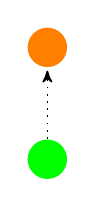
\begin{tikzpicture}[->,>=stealth',shorten >=1pt,auto,node distance=2cm,
                    semithick]

  \node[state, fill = green, draw = none,minimum size=.5cm] (A)                    {};
  \node[state, fill = orange, draw = none,minimum size=.5cm]         (C) [above =.9cm of A] {};

  \path[dotted] (A) edge              (C);

      \end{tikzpicture}
    \caption{Inflorescence meristem remaining an inflorescence meristem and generating a floral meristem}
  \end{subfigure}
        \caption{Meristem transitions in plants with determinate inflorescences.}
\end{figure}

% new figure
\begin{figure}[hbt!]
  \begin{subfigure}{.25\textwidth}
  \centering
    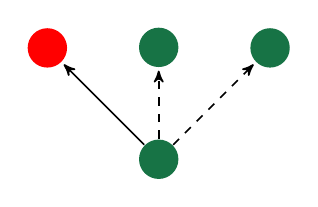
\begin{tikzpicture}[->,>=stealth',shorten >=1pt,auto,node distance=2cm,
                    semithick]
  \tikzstyle{every state}=[draw=none]

  \node[state, fill=darkspringgreen,minimum size=.5cm] 	     (A)                    {};
  \node[state, fill=red,minimum size=.5cm]         (B) [above left of=A] {};
  \node[state, fill=darkspringgreen,minimum size=.5cm]         (C) [above right of=A] {};
  \node[state, fill=darkspringgreen,minimum size=.5cm] 	     (D) [above = .9cm of A]                   {};

  \path[dashed] (A) edge              (D)
            	edge               (C);
  \path[->] (A) edge (B);

      \end{tikzpicture}
          \caption{Primary meristem transitioning to one vegetative meristem and generating two primary meristems.} 
  \end{subfigure}
              \hspace{\fill}
             \begin{subfigure}{.25\textwidth}
    \centering
    \centering

      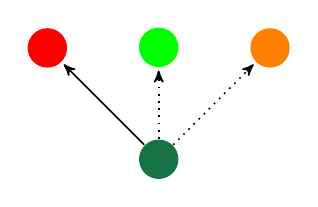
\begin{tikzpicture}[->,>=stealth',shorten >=1pt,auto,node distance=2cm,
                    semithick]
  %\tikzstyle{every state}=[fill=red,draw=none,text=white]

  \node[state, fill = darkspringgreen, draw = none,minimum size=.5cm] (A)                    {};
  \node[state, fill = red, draw = none,minimum size=.5cm]         (B) [above left of=A] {};
  \node[state, fill = orange, draw = none,minimum size=.5cm]         (C) [above right of=A] {};
  \node[state, fill=green, draw = none,minimum size=.5cm] 	     (D) [above =.9cm of A]                   {};

  \path[dotted] (A) edge              (D)
            	edge               (C);
  \path[->] (A) edge (B);

      \end{tikzpicture}
    \caption{Primary meristem transitioning to one vegetative meristem, and generating inflorescence and floral meristems.}
      \end{subfigure}
          \hspace{\fill}
      \begin{subfigure}{.25\textwidth}
% stem cell expansion
\centering
% stem cell expansion
      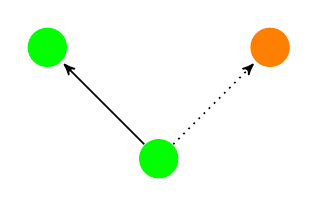
\begin{tikzpicture}[->,>=stealth',shorten >=1pt,auto,node distance=2cm,
                    semithick]
  %\tikzstyle{every state}=[fill=red,draw=none,text=white]

  \node[state, fill = green, draw = none,minimum size=.5cm] (A)                    {};
  \node[state, fill = green, draw = none,minimum size=.5cm]         (B) [above left of=A] {};
  \node[state, fill = orange, draw = none,minimum size=.5cm]         (C) [above right of=A] {};

  \path[dotted] (A) edge              (C);
  \path (A) edge		     (B);

      \end{tikzpicture}
    \caption{Inflorescence meristem remaining an inflorescence meristem and generating a floral meristem}
  \end{subfigure}
        \caption{Meristem transitions in plants with determinate inflorescences.}
\end{figure}

I use these types of divisions/transitions to summarize the meristem dynamics for plants with determinate inflorescences in a system of equations with constraints (Equation \ref{eqn:de-determinate} and \ref{eqn:constraints-determinate}) and a state diagram (Figure \ref{fig:state-determinate}). In this model, $P$, $V$, $I$, and $F$ are the populations of primary, vegetative, inflorescence, and floral meristems, respectively. Primary meristems divide at a rate $\beta_1$. Inflorescence meristems divide at a rate $\beta_2$, and are thus converted to floral meristems at a rate $\beta_2$. Each division by an inflorescence meristem produces one inflorescence meristem and one floral meristem. The probability that a primary meristem divides into two primary meristems (branch and axillary meristem) and a vegetative meristem is given by the control function, $p(t)$. The probability that a primary meristem divides into a vegetative meristem, inflorescence meristem, and a floral meristem is given by $1-p(t)$. 

To summarize Figure \ref{fig:state-determinate}, panel (A) occurs proportional to the number of primary meristems at a rate $\beta_1 p(t)$. Panel (B) occurs proportional to the number of primary meristems at a rate $\beta_1 (1-p(t))$. Panel (C) occurs proportional to the number of inflorescence meristems at a rate $\beta_2$.

The goal of this optimization problem is to maximize $F$. The variable in the model is $T$, the length of the season. The model is described by the following system of differential equations:
%
\begin{align}
\dot{P} & = 2 \beta_1 p(t) P - \beta_1 p(t) P - ( 1-p(t) ) \beta_1 P \nonumber \\
\dot{V} & = \beta_1 p(t) P + ( 1-p(t) ) \beta_1 P \nonumber \\
\dot{I} & = \beta_1 ( 1-p(t) ) P \nonumber \\ %+ \beta_2 I \nonumber \\
\dot{F} & = \beta_1 ( 1-p(t) ) P + \beta_2 I
\label{eqn:de-determinate}
\end{align}

\noindent subject to
%
\begin{align}
0 \leq & p(t) \leq 1 \nonumber \\
0 & < P \nonumber \\
0 & \leq I \nonumber \\
0 & \leq F
\label{eqn:constraints-determinate}
\end{align}

\begin{figure}[hbt!]
\centering
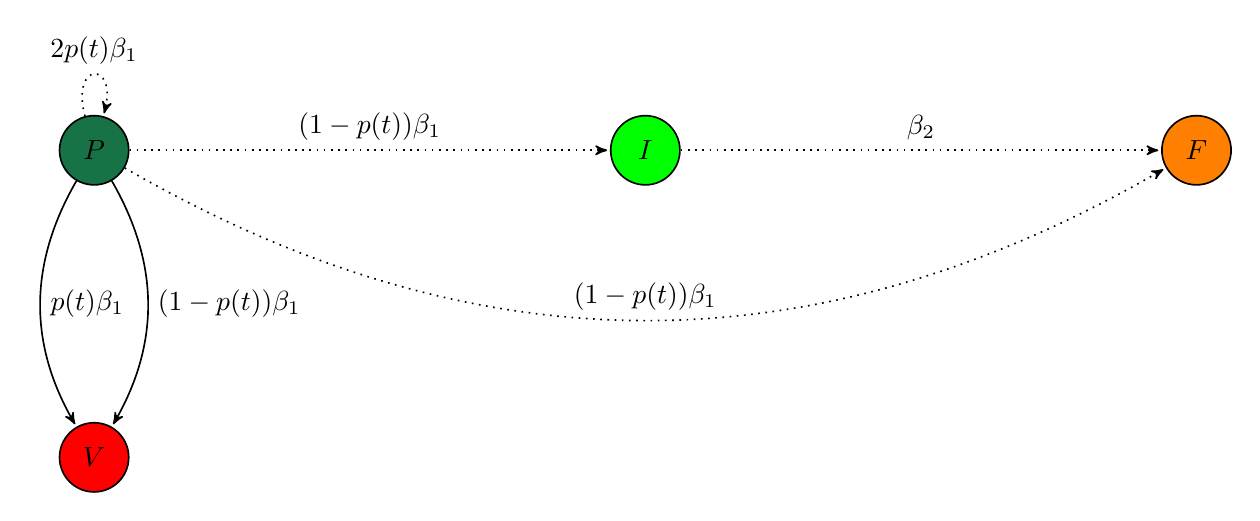
\begin{tikzpicture}[->,>=stealth',shorten >=1pt,auto,node distance=7cm,
                    semithick]
  \tikzstyle{every state}=[draw]    
   \node [state, fill=darkspringgreen] (a) { $P$ };
    \node [state, fill=green] (c) [right of=a] {$I$};
    \node [state, fill=orange] (d) [right of=c] {$F$};    
    \node [state, fill=red] (e) [below = 3cm of a] {$V$};    
    
    \path[dotted, ->] (a) edge node {$(1-p(t))\beta_1 $} (c);
    \path[dotted] (a) edge [loop above] node {$ 2 p(t)  \beta_1$} (a);
    %\path[dotted] (c) edge [loop above] node {$\beta_2$} (c);   
    \path[dotted, ->] (c) edge node {$\beta_2$} (d);    
    \path[dotted] (a) edge[bend right] node {$( 1-p(t) ) \beta_1 $} (d);
    \path (a) edge [bend right] node {$ p(t)  \beta_1$} (e);
    \path (a) edge [bend left] node {$ ( 1-p(t) ) \beta_1 $} (e);

\end{tikzpicture}
  \caption{State diagram describing the dynamics for plants with determinate inflorescences.}
  \label{fig:state-determinate}
\end{figure}

The equation $\dot{P}  = 2 \beta_1 p(t) P - \beta_1 p(t) P - ( 1-p(t) ) \beta_1 P $ describes how primary meristems that divide into two primary meristems add to the pool $P$ in proportion to size of the pool of primary meristems. These divisions also add to the vegetative meristem pool $V$. The process here is that a primary meristem unit becomes a vegetative meristem, and gives rise to two new primary meristems. Primary meristems are lost from the primary meristem pool when divisions give rise to inflorescence and floral meristems.

The equation $ \beta_1 p(t) P + ( 1-p(t) ) \beta_1 P $ describes the dynamics of the vegetative meristems. Primary meristems contribute to the vegetative pool when primary meristems propagate. The transition from primary to vegetative meristems is a proper flow. Primary meristems also contribute to the vegetative pool when primary meristems divide into inflorescence and floral meristems. This is also a flow.
 
The equation $\dot{I} = \beta_1 ( 1-p(t) ) P $ describes the dynamics of the inflorescence meristems. Primary meristems contribute to inflorescence meristems when they; this happens with probability $1-p(t)$ and proportional to the primary meristem pool $P$. 

The equation $\dot{F} = \beta_1 ( 1-p(t) ) P + \beta_2 I$ describes the dynamics of the floral meristems. Primary meristems contribute to floral meristems with probability $1-p(t)$ and proportional to the primary meristem pool $P$. Inflorescence divisions also contribute to floral meristems and occur proportional to the size of the inflorescence meristem pool.

% \textcolor{red}{SPE: The differential equations are inconsistent about the fate of primary meristems that divide. The first line of equation 1 says that each division of a P meristem produces one new P meristem, not two of them. This is right if the process is one P meristem dividing into two, rather than one parent producing two offspring while the parent survives. However, if the process is one meristem dividing into two (and the parent does not survive) then each of the divisions depicted in Figure 1B results in the loss of one P meristem, and that would produce an additional term negative term in the first line of equation 1: loss of a P meristem every time one of them divides into an I and an F. Absence of that term corresponds to the parent surviving. GS: Each division of a P meristem produces 2 new P meristems if there is branching. So I need to change the first line of equation 1 to correctly state that a parent P meristem survives. OR I need to move that parent P meristem to an additional pool that is now photosynthetically active and constrains the rate of meristem division. }

\subsection{Model description}
Qualitatively, this model describes the accumulation of primary meristems through division at the shoot apical meristem (SAM). Without further modification to the model, all primary meristems have active SAMs (can produce further primary meristems through division). Primary meristems that are converted to inflorescence meristems or floral meristems can not revert to primary meristems. Inflorescence meristems divide and produce inflorescence and floral meristems, but can not produce more vegetative axillary meristems. For values of $p(t)=0$, plants produce vegetative, inflorescence, and floral meristems in proportion to the available primary meristem pool. 

There are two rates in the model: the rate of primary meristem division and the rate of inflorescence meristem division. High rates of primary meristem division ($\beta_1$) correspond to morphologies with short internodes (e.g. rosettes) or high levels of branching. Low rates of primary meristem division correspond to morphologies with long internodes and low levels of branching. High rates of inflorescence meristem division ($\beta_2$) correspond to tightly packed inflorescences. Low rates of inflorescence meristem division correspond to spaced floral meristems. 

In this model, committing a primary meristem to flowering consumes the branch. The process produces a terminal flower and inflorescence meristem; this structure can be iterated but can't revert to producing primary meristems. This should show up in the model because the decision for total asymmetric branching ($p(t)=0$) will convert primary meristems to inflorescence and floral meristems. This means that once all meristems are committed to flowering, the only way in which reproductive biomass (i.e. floral meristems) will get added is by division of the inflorescence meristems. 

\subsection{Equations}

The optimal control problem we are interested in is
%
\begin{align}
\max_{u} &  \int_0^T \log( F(t) ) dt \nonumber \\
\mathrm{subject\ to\ } 
& \dot{P}  = 2 \beta_1 p(t) P - \beta_1 p(t) P - ( 1-p(t) ) \beta_1 P \nonumber \\
& \dot{V} = \beta_1 p(t) P + ( 1-p(t) ) \beta_1 P \nonumber \\
& \dot{I}  = \beta_1 ( 1-p(t) ) P \nonumber \\ 
& \dot{F}  = \beta_1 ( 1-p(t) ) P + \beta_2 I
 \nonumber \\ 
& 0 < P,\ 0 \leq V,\ 0 \leq I,\ 0 \leq F, \nonumber\\
& 0 \leq p(t) \leq 1,\ 0 \leq q(t) \leq 1. \nonumber
\end{align}

If we set $\beta_1, \beta_2$ to be functions of vegetative biomass, we write the system of equations:
%
\begin{align}
& \dot{P}  = 2 [q(t) V] p(t) P - [q(t) V] p(t) P - ( 1-p(t) ) [q(t) V] P \nonumber \\
& \dot{V} = [q(t) V] p(t) P + ( 1-p(t) ) [q(t) V] P \nonumber \\
& \dot{I}  = [q(t) V] ( 1-p(t) ) P \nonumber \\ 
& \dot{F}  = [q(t) V] ( 1-p(t) ) P + [1-q(t)] V I
\end{align}

The Hamiltonian here is:
%
\begin{align}
H & = \log( F ) + \bm{\lambda}^T [P\ V\ I\ F] \\
& = \log( F ) + \left(PV \left(2\lambda_1 -\lambda_3-\lambda_4 \right)p+\left(P-I\right)V\lambda_4+PV (
\lambda_3+\lambda_2-\lambda_1) \right)q+I
 V\lambda_4
\end{align}

If season length is uniformly distributed over, season length factors out of the objective function. The objective function is independent of the control . For this problem, the optimality condition is 
%
\begin{align}
\frac{\partial H}{\partial p} & = PV (2\lambda_1 - \lambda_3-\lambda_4 )q = 0\ \mathrm{at}\ u^* \nonumber \\
\frac{\partial H}{\partial q} & = PV( 2 \lambda_1 - \lambda_3- \lambda_4 )p+(P-I)V \lambda_4+PV (
 \lambda_3+\lambda_2-\lambda_1) = 0\ \mathrm{at}\ u^*.
\end{align}

The transversality condition is
\begin{align}
\lambda_1(T) = \lambda_2(T) = \lambda_3(T) = \lambda_4(T) = 0.
\end{align}

The adjoint equations are
%
\begin{align}
&-\frac{\partial H}{\partial P} = \dot{\lambda_1}  = -( V(2 \lambda_1 - \lambda_3 - \lambda_4)p+V ( \lambda_4+\lambda_3+ \lambda_2 - \lambda_1) )q \nonumber \\
&-\frac{\partial H}{\partial V} = \dot{\lambda_2}  =  -( P ( 2 \lambda_1 - \lambda_3 - \lambda_4 ) p+ ( P-I ) \lambda_4 +P ( \lambda_3+ \lambda_2- \lambda_1) ) q - I \lambda_4 \nonumber \\
&-\frac{\partial H}{\partial I} = \dot{\lambda_3}  = V \lambda_4 q - V \lambda_4  \nonumber \\
&-\frac{\partial H}{\partial F} = \dot{\lambda_4}  = - \frac{1}{F}
\end{align}





\section{Indeterminate inflorescences}

In plants with indeterminate inflorescences, the inflorescence meristem only produces flowers at axillary positions. For example, in \textit{Arabidopsis} the primary shoot meristem converts to an inflorescence meristem that bears floral meristems in axillary positions \cite{bradley1997}.

I describe the developmental decisions in a plant with indeterminate inflorescences using four types of divisions ((Figure \ref{fig:transitions-indeterminate}). First, a primary meristem can divide at the shoot apical meristem to give rise to two primary meristems: the main branch and an axillary bud. These divisions lead to a vegetative, branching architecture. Second, a primary meristem can divide at the shoot apical meristem to give rise to a primary meristem and an inflorescence meristem: a branch and an inflorescence. These divisions  produce either (1) an axillary inflorescence or (2) an inflorescence along the main branch and a vegetative, primary meristem that can continue branching. Third, a primary meristem can divide at the shoot apical meristem to give rise to two inflorescence meristems. Fourth, an inflorescence meristem can divide to give rise to an inflorescence meristem and a floral meristem. Inflorescence meristems have a single fate: they produce a branch with floral meristems in axillary positions.

% indeterminate growth
\begin{figure}[hbt!]
  \begin{subfigure}[h]{.2\textwidth}
    \centering
    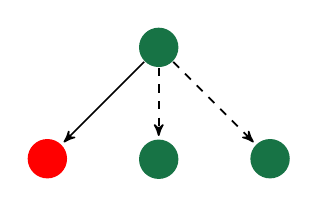
\begin{tikzpicture}[->,>=stealth',shorten >=1pt,auto,node distance=2cm,
                    semithick]
  \tikzstyle{every state}=[draw=none]

  \node[state, fill=darkspringgreen,minimum size=.5cm] 	     (A)                    {};
  \node[state, fill=red,minimum size=.5cm]         (B) [below left of=A] {};
  \node[state, fill=darkspringgreen,minimum size=.5cm]         (C) [below right of=A] {};
  \node[state, fill=darkspringgreen,minimum size=.5cm] 	     (D) [below =.9cm of A]                   {};

  \path[dashed] (A) edge              (D)
            	edge               (C);
  \path[->] (A) edge (B);

      \end{tikzpicture}
          \caption{Primary meristem transitioning to one vegetative meristem and generating two primary meristems.} 
  \end{subfigure}
            \hspace{\fill}  
  \begin{subfigure}[h]{.2\textwidth}
    \centering
      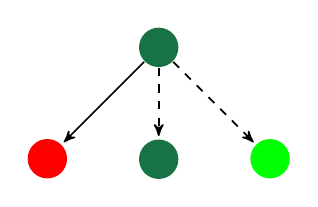
\begin{tikzpicture}[->,>=stealth',shorten >=1pt,auto,node distance=2cm,
                    semithick]
  \tikzstyle{every state}=[draw=none]

  \node[state, fill=darkspringgreen,minimum size=.5cm] 	     (A)                    {};
  \node[state, fill=red, minimum size=.5cm]         (B) [below left of=A] {};
  \node[state, fill=green, minimum size=.5cm]         (C) [below right of=A] {};
  \node[state, fill=darkspringgreen,minimum size=.5cm] 	     (D) [below =.9cm of A]                   {};

  \path[dashed] (A) edge              (D)
            	edge               (C);
  \path[->] (A) edge (B);

      \end{tikzpicture}
          \caption{Primary meristem transitioning to one vegetative meristem and generating primary and inflorescence meristems.} 
  \end{subfigure} 
              \hspace{\fill}
             \begin{subfigure}[h]{.2\textwidth}
    \centering
    \centering

      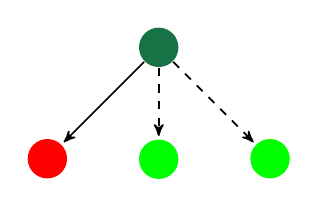
\begin{tikzpicture}[->,>=stealth',shorten >=1pt,auto,node distance=2cm,
                    semithick]
  \tikzstyle{every state}=[draw=none]

  \node[state, fill=darkspringgreen,minimum size=.5cm] 	     (A)                    {};
  \node[state, fill=red, minimum size=.5cm]         (B) [below left of=A] {};
  \node[state, fill=green, minimum size=.5cm]         (C) [below right of=A] {};
  \node[state, fill=green,minimum size=.5cm] 	     (D) [below =.9cm of A]                   {};

  \path[dashed] (A) edge              (D)
            	edge               (C);
  \path[->] (A) edge (B);

      \end{tikzpicture}
          \caption{Primary meristem transitioning to one vegetative meristem and generating inflorescence meristems.} 
  \end{subfigure} 
            \hspace{\fill}
  \begin{subfigure}[h]{.2\textwidth}
    \centering
    \centering
% stem cell expansion

% stem cell expansion
      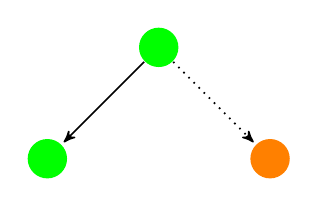
\begin{tikzpicture}[->,>=stealth',shorten >=1pt,auto,node distance=2cm,
                    semithick]
  %\tikzstyle{every state}=[fill=red,draw=none,text=white]

  \node[state, fill = green, draw = none,minimum size=.5cm] (A)                    {};
  \node[state, fill = green, draw = none,minimum size=.5cm]         (B) [below left of=A] {};
  \node[state, fill = orange, draw = none,minimum size=.5cm]         (C) [below right of=A] {};

  \path[dotted] (A) edge              (C);
  \path (A) edge		     (B);

      \end{tikzpicture}
    \caption{Inflorescence meristem remaining an inflorescence meristem and generating a floral meristem}
  \end{subfigure}\
        \caption{Meristem transitions in plants with indeterminate inflorescences.}
\end{figure}

I use these types of divisions/transitions to summarize the meristem dynamics for plants with indeterminate inflorescences in a system of equations with constraints (Equation \ref{eqn:de-indeterminate} and \ref{eqn:constraints-indeterminate}) and a state diagram (Figure \ref{fig:state-indeterminate}). In this model, $P$, $V$, $I$, and $F$ are the populations of primary, vegetative, inflorescence, and floral meristems, respectively. 

\subsection{Description of diagram}

The division shown in Figure \ref{fig:transitions-indeterminate}A occurs at rate $\beta_1 p(t)$. The rate is the product of $\beta_1$, the ..., and $p(t)$, the probability with which the division shown in Figure \ref{fig:transitions-indeterminate}A occurs. It results in the net gain of one primary meristem and gain of one vegetative meristem. The differential equations corresponding to this are:
%
\begin{align}
\dot{P} & = 2 \beta_1 p(t)  P - \beta_1 p(t) P = \beta_1 p(t) P \nonumber \\
\dot{V} & = \beta_1 p(t)  P      \nonumber \\
\dot{I} & = 0  \nonumber \\
\dot{F} & = 0
\end{align}
%
The division shown in Figure \ref{fig:transitions-indeterminate}B occurs at a rate $\beta_1 q(t)$. The rate is the product of $\beta_1$, the ..., and $q(t)$, the probability with which the division shown in Figure \ref{fig:transitions-indeterminate}B occurs. It results in the gain of one vegetative meristem and the gain of one inflorescence meristem. The differential equations corresponding to this are:
%
\begin{align}
\dot{P} & = 0 \nonumber \\
\dot{V} & = \beta_1 q(t) P      \nonumber \\
\dot{I} & =  \beta_1 q(t) P \nonumber \\
\dot{F} & = 0
\end{align}
%

The division shown in Figure \ref{fig:transitions-indeterminate}C occurs at a rate $\beta_1 r(t)$. The rate is the product of $\beta_1$, the ..., and $r(t)$, the probability with which the division shown in Figure \ref{fig:transitions-indeterminate}C occurs. It results in the net gain of two inflorescence meristems, gain of one vegetative meristem, and the loss of one primary meristem. The differential equations corresponding to this are:
%
\begin{align}
\dot{P} & = - \beta_1 r(t) P \nonumber \\
\dot{V} & = \beta_1 r(t)  P      \nonumber \\
\dot{I} & =  2 \beta_1 r(t) P \nonumber \\
\dot{F} & = 0
\end{align}
%

The division shown in Figure \ref{fig:transitions-indeterminate}D occurs at a rate $\beta_2 $. It results in the net gain of one floral meristem. The differential equations corresponding to this are:
%
\begin{align}
\dot{P} & = 0 \nonumber \\
\dot{V} & = 0      \nonumber \\
\dot{I} & =  0 \nonumber \\
\dot{F} & = \beta_2 I
\end{align}
%

The full system of differential equations for the system thus becomes:
%
\begin{align}
\dot{P} & = \beta_1 (p(t) - r(t)) P  \nonumber \\
\dot{V} & = \beta_1 (p(t) + q(t) + r(t) ) P     \nonumber \\
\dot{I} & =  \beta_1 (q(t) + 2 r(t) ) \nonumber \\
\dot{F} & = \beta_2 I
\label{eqn:de-indeterminate}
\end{align}
%
I assume that 
%
\begin{align}
p(t) + q(t) + r(t) \leq 1
\end{align}
Because they are probabilities, the controls $p(t)$, $q(t)$, and $r(t)$ are constrained on $[0,1]$. The difference between controls (e.g. $p(t) - r(t)$) is not constrained and can be negative. For example, when the probability of division into two inflorescence meristems is greater than the probability of division into two primary meristems, the value of $\dot{P}<0$ and corresponds to a decrease in the size of the primary meristem pool. If all primary meristem divisions are like in Panel A, $\dot{I} = 0$. If $p + q + r < 1$ at any point, than it's beneficial to increase p.

The goal of this optimization problem is to maximize $F$. The variable in the model is $T$, the length of the season. The model is described by the system of differential equations above \ref{eqn:de-indeterminate} and subject to 
%
\begin{align}
0 \leq & p(t) \leq 1,\ 0 \leq q(t) \leq 1,\ 0 \leq r(t) \leq 1,  \nonumber \\
0 & < P,\ 0 \leq V,\ 0 \leq I,\ 0  \leq F 
\label{eqn:constraints-indeterminate}
\end{align}

I also tried to summarize the dynamics in a state diagram:

\begin{figure}[hbt!]
\centering
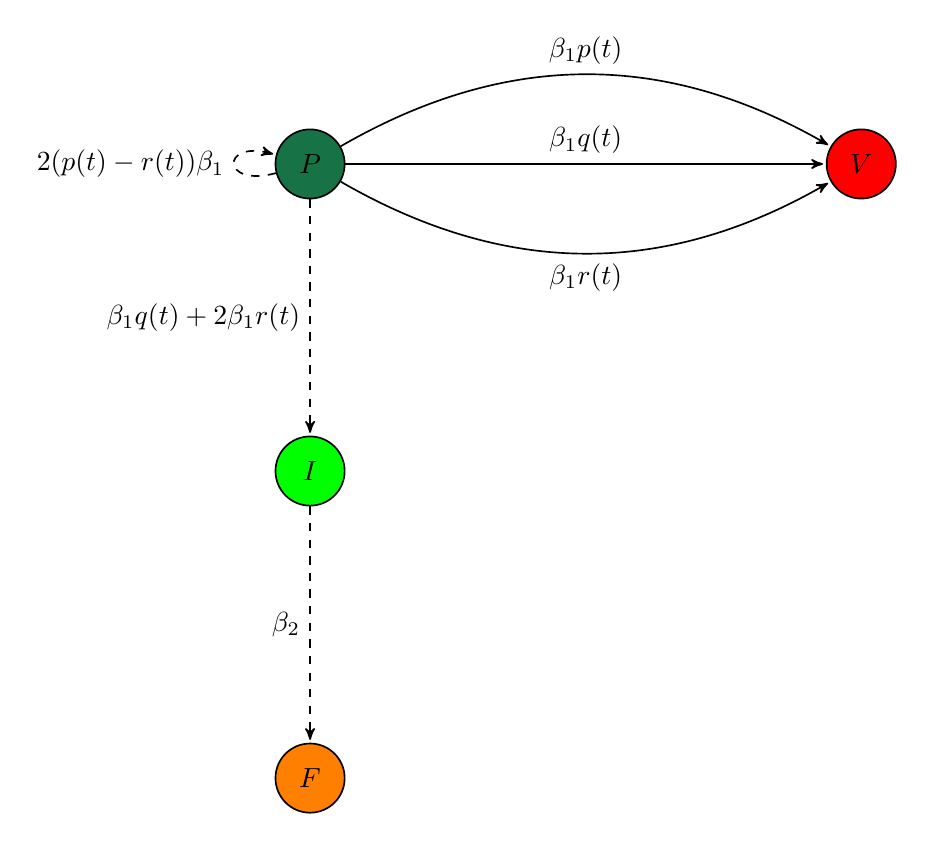
\begin{tikzpicture}[->,>=stealth',shorten >=1pt,auto,node distance=7cm,
                    semithick]
  \tikzstyle{every state}=[draw]    
   \node [state, fill=darkspringgreen] (a) { $P$ };
    \node [state, fill=red] (e) [right of=a] {$V$};
    
    
    \node [state, fill=green] (b) [below = 3cm of a] {$I$};    
    \node [state, fill=orange] (c) [below = 3cm of b] {$F$};    

    \path[dashed, ->] (a) edge node [left] {$ \beta_1 q(t) + 2 \beta_1 r(t) $} (b);
    \path[dashed] (a) edge [loop left] node {$2 ( p(t) - r(t) )\beta_1$} (a);
  %  \path (c) edge [loop above] node {$\beta_2$} (c);   
    \path[dashed, ->] (b) edge node [left] {$\beta_2$} (c);    
       \path (a) edge [bend right] node [below] {$  \beta_1 r(t)$} (e);
    \path (a) edge [bend left] node [above]  {$\beta_1  p(t) $} (e);
        \path (a) edge node  {$  \beta_1 q(t) $} (e);

    \end{tikzpicture}
  \caption{State diagram describing the dynamics for plants with indeterminate inflorescences.}
  \label{fig:state-indeterminate}
\end{figure}

The equation $\dot{P}  = \beta_1 (p(t) - q(t)) P$ describes how primary meristems that divide into two primary meristems add to the pool $P$, and primary meristems that divide into two inflorescence meristems subtract from the pool $P$. 

The equation $\dot{I} = \beta_1 (1-p(t)- q(t) ) P + 2 \beta_1 q(t) P + \beta_2 I $ describes how primary meristems contribute to inflorescence meristems when they divide asymmetrically (i.e. do not divide into two primary meristems or into two inflorescence meristems); this happens with probability $1-p(t)-q(t)$ and when they divide into two inflorescence meristems with probability $q(t)$. Because the primary meristem divides into two inflorescence meristems, the value is doubled in the equation. Finally, inflorescence divisions occur proportional to the size of the inflorescence meristem pool.

The equation $\dot{F} = \beta_2 I$ describes how inflorescence meristems divide proportional to the size of the inflorescence meristem pool. Each division produces a floral meristem.

\subsection{Model description - NEED TO UPDATE}

Qualitatively, this model describes the accumulation of primary meristems through division at the shoot apical meristem. Without further modification to the model, all primary meristems have active SAMs (can produce further primary meristems through division). Primary meristems that are converted to inflorescence meristems can not be reverted to primary meristems. These inflorescence meristems can divide and produce floral meristems but can not produce more axillary meristems with the potential to produce more inflorescence meristems. For values of $p(t)=q(t)=0$, plants produce both primary and inflorescence meristems. 

There are two rates in the model: the rate of primary meristem division and the rate of inflorescence meristem division. High rates of primary meristem division ($\beta_1$) correspond to morphologies with short internodes (e.g. rosettes) or high levels of branching. Low rates of primary meristem division correspond to morphologies with long internodes and low levels of branching. High rates of inflorescence meristem division ($\beta_2$) correspond to tightly packed inflorescences. Low rates of inflorescence meristem division correspond to spaced inflorescences.

Another point that I need to elaborate on is how vegetative pools and meristem pools are related. See Korner 2015 for one opinion, as well as Fatichi for a complementary view. Some way of modeling this as source/sink dynamics (cf. Neubert?)

\subsection{Optimal control problem and goals}


\subsection{Analysis of optimal control problem}

\subsection{Numerical algorithm}


\clearpage
\newpage

\section{Results}

\subsection{Optimal strategies}

I will use the models to determine whether including differentiation and growth of meristems reduces the likelihood of obtaining a strategy with an instantaneous switch \cite{cohen1971}. Put another way, are graded allocation strategies optimal when vegetative and reproductive growth are coupled \cite{fox1992a}?

\subsection{Development patterns}

I will ask when plants are more likely to be resource versus meristem limited depending on their relative propensity for branching and resource use efficiencies. Specifically, I will focus on how the optimal strategy changes as the probability of branching and resource use efficiency varies jointly.

 \begin{figure}[!h]
       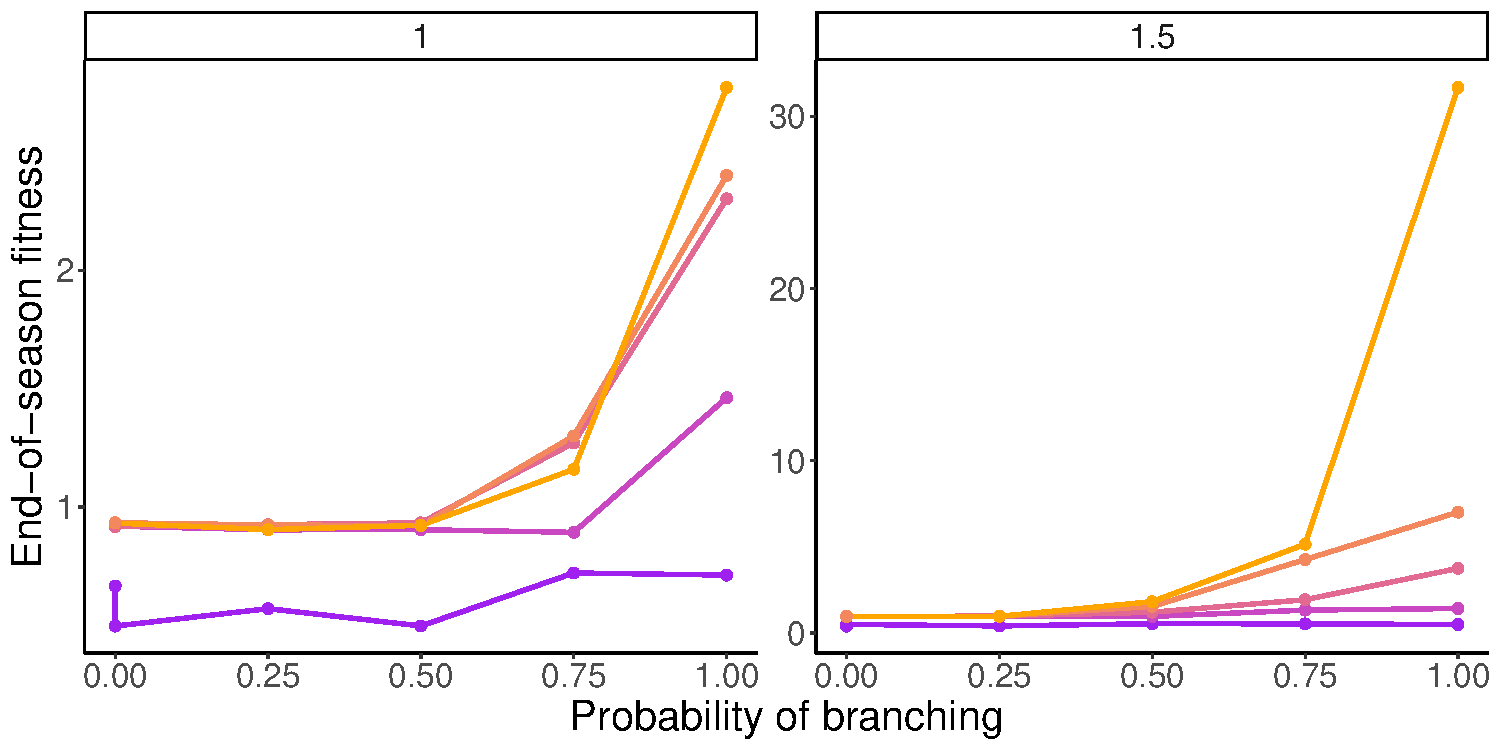
\includegraphics[page=1,width=.5\textwidth]{../figures/resources2.pdf}  
       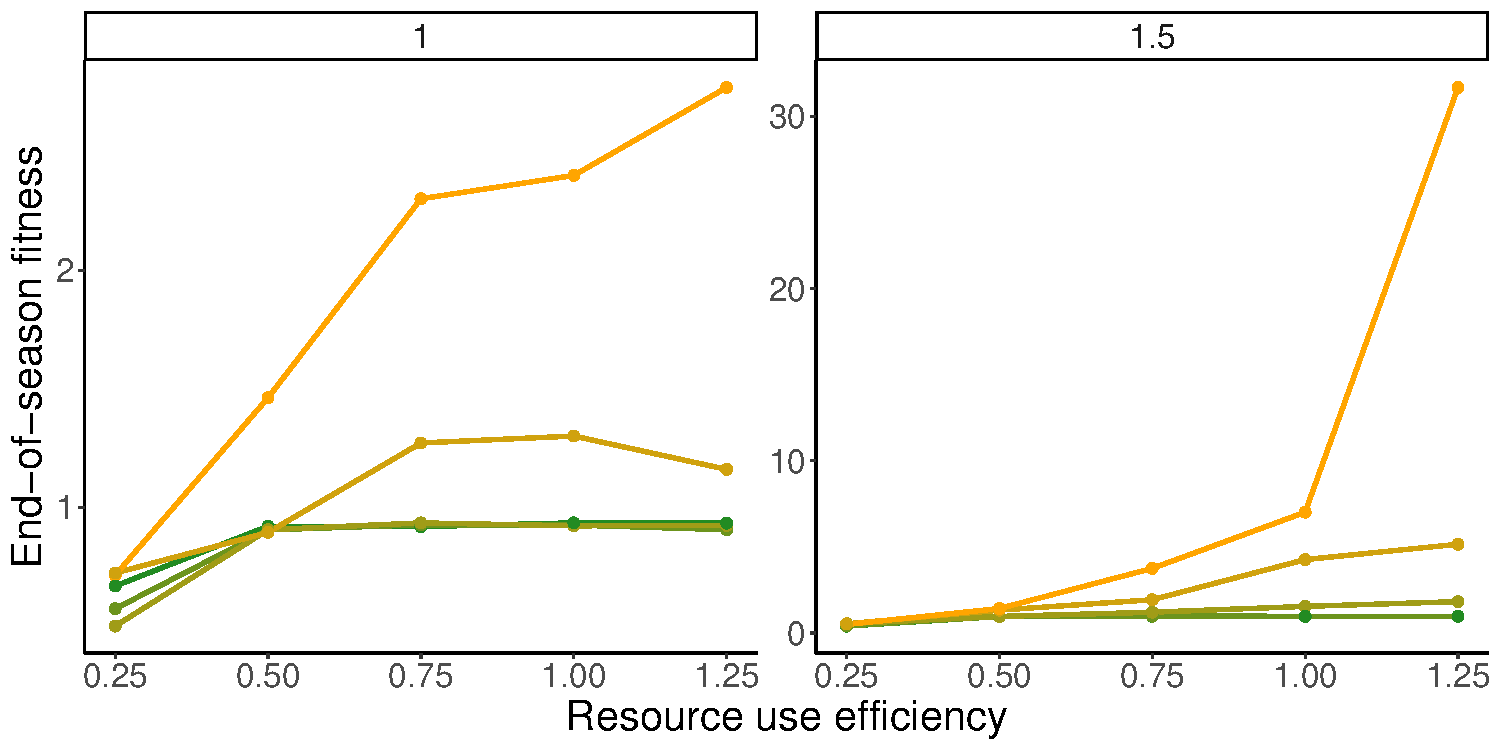
\includegraphics[page=1,width=.5\textwidth]{../figures/resources3.pdf}  
%    \caption[left]{  }
\end{figure}

Steve and I have discussed that the degree of resource or meristem limitation would be best analyzed in terms of sensitivities, rather than the end-of-season fitnesses I have presented above. 

\subsection{Environmental variation}

I will ask when plants are more likely to be resource versus meristem limited. Specifically, I will focus on how the optimal strategy changes with environmental variation; are plants likely to be meristem limited in scenarios with high levels of uncertainty about season length as a result of selection for the ability to capitalize on longer, if infrequent, seasons?

In resource-only models (e.g. \cite{king1982a}), increasing variation in season length increases the proportion of the season in which the singular, graded control is optimal.

 \begin{figure}[!h]
       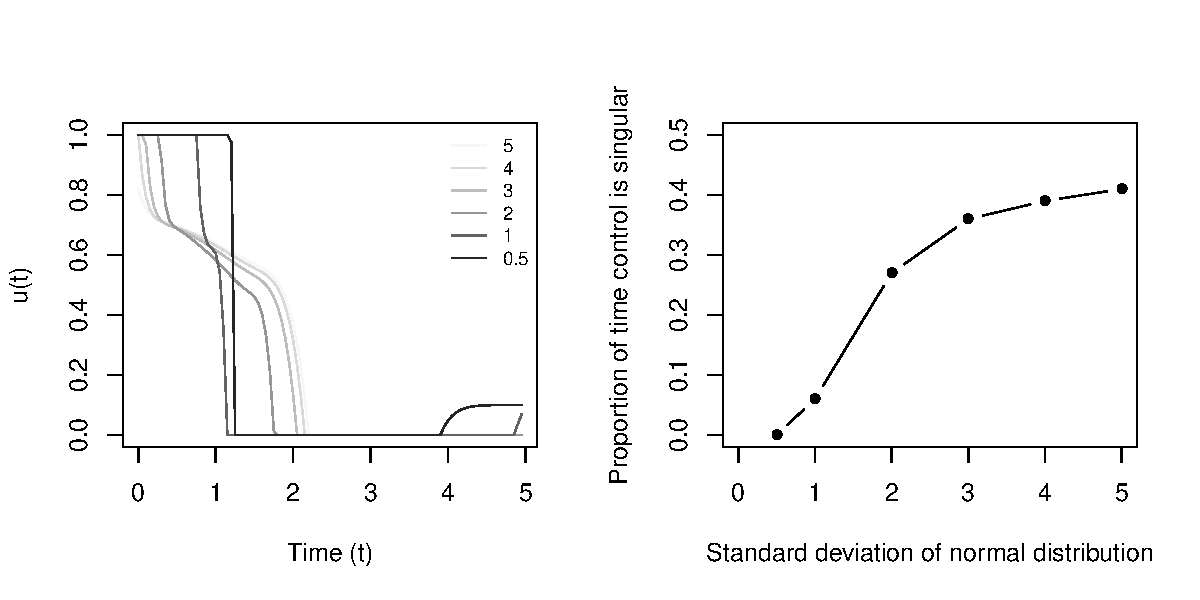
\includegraphics[page=1,width=.75\textwidth]{../figures/kingRoughgardenNormalSummary.pdf}  
 %   \caption{  }
\end{figure}

Below, I've included a plot of how end of-season fitness changes as a function of season length under a uniform distribution of season lengths for varying probabilities of branching. 

 \begin{figure}[!h]
       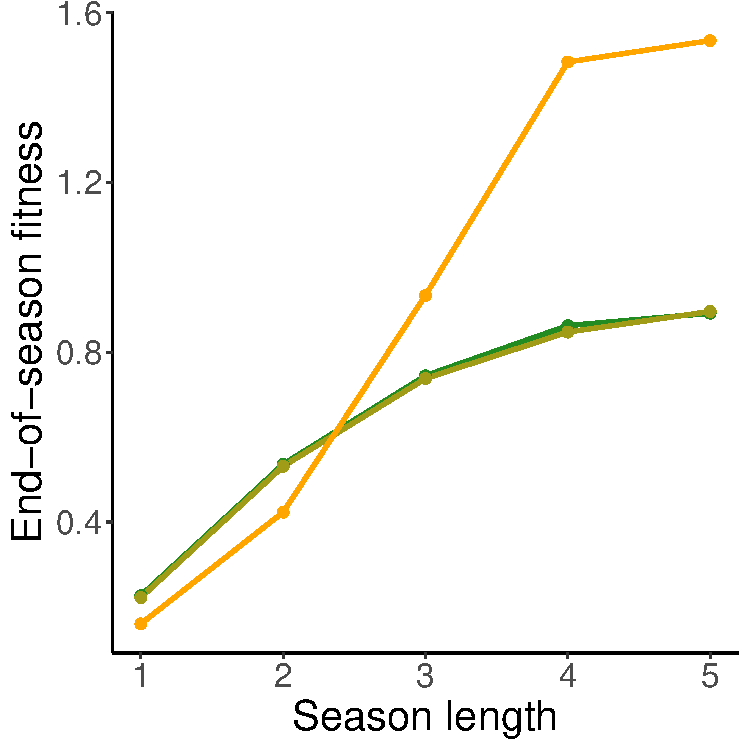
\includegraphics[page=1,width=.3\textwidth]{../figures/season.pdf}  
  %  \caption{  }
\end{figure}


%%%%%%%%%%%%%%%%%%%%%%%%%%%%%%%%%%%%%%%%%%%%%%%%%%%%
% BIBLIOGRAPHY
%%%%%%%%%%%%%%%%%%%%%%%%%%%%%%%%%%%%%%%%%%%%%%%%%%%%
\clearpage
\bibliographystyle{/Users/gregor/Dropbox/bibliography/styleFiles/ecology} 
%\bibliography{/Users/gregor/Dropbox/bibliography/optimal-control-lit}
\bibliography{/Users/gregor/Dropbox/bibliography/chapter-2}

\clearpage
%%%%%%%%%%%%%%%%%%%%%%%%%%%%%%%%%%%%%%%%%%%%%%%%%%%%
% SUPPLEMENTARY MATERIAL
%%%%%%%%%%%%%%%%%%%%%%%%%%%%%%%%%%%%%%%%%%%%%%%%%%%%
\section*{Supplementary material}

\subsection*{Background for hypotheses.} Explanation of key papers that motivate the hypotheses in this manuscript. The document describes results from these papers that are relevant to understanding and interpreting the data in this manuscript. Link to document: \dots

\subsection*{Numerical methods.} Description of numerical methods used to solve the optimal control problems. Includes outline of algorithm and code for a generic version of the optimal control problem. Link to document: \dots

\subsection*{Resource allocation model.} Explanation of models representing plant life history as a resource allocation problem, and analysis of how these models connect to the ones presented in this manuscript. Link to document: \dots

\subsection*{Analysis of optimal control problem.} Presents an analysis of the optimal control problem. Link to document: \dots


\end{document}